
\chapter{アプローチ}
本研究ではドライブレコーダーの映像から自動車を検出,車間距離を推定し,渋滞しているか否かを判断するシステムDepth2Jamを提案する.
本章では,自動車の検出と車間距離を推定する手法とそのネットワーク構造について述べる.

\section{設計}
本研究では,汎用性を重視するためにドライブレコーダーから得られる情報のみを利用する.
渋滞の定義の項でも述べたが,渋滞を推定するためには速度が重要だが,ドライブレコーダーと自動車の速度を同期させるためには専用の取り付け工事が必要であり,また車の種類や自動車メーカーによって内部構造は異なっている.
また,映像から速度を推定する方法も手法の一つとして考えられるが,映像から速度を出すためには相対距離の算出が必要であり,リアルタイムの情報が求められているこの研究では相対速度を計算する処理は処理時間を増やす原因を作ると同時に,映像から正確な速度情報を算出することは非常に困難である.
また,速度センサーを搭載して速度を求める方法も考えられ,加速度センサーの使用が考えられる.
しかし,現状加速度センサーが搭載されている市販のドライブレコーダーは存在しないため,状況が限られてしまい,汎用性が担保できない問題が発生する.
また,加速度センサーが搭載されているスマートフォンを自動車に取り付けて速度推定を行う方法も考えられる.
一般的に,速度は加速度を積分することでその時々の速度を推定することができるが,不良積分が多く発生してしまう恐れがあると同時に,物体検出,速度推定に加えてそのような加速度センサーデータから速度を計算すると機械が処理するものが多くなり,映像の処理におけるFPSが低下する恐れがある.
このFPSの低下はリアルタイムでの処理を目指すこの研究において重大な欠陥となってしまう.

さらに,GPSを用いて渋滞を推定する方法もあるが,ドライブレコーダー等の映像記録装置は実際に映像を取得できる利点があるのに対して,GPSは位置情報データーを取得するため,得られる情報に限りがある.
その上,GPSのみで渋滞情報を取得する方法は例えばGPSを搭載した電子機器を複数自動車に持ち込むと,実際には渋滞していないのにもかかわらず,渋滞していると出力してしまうような事例がある\cite{create_jam}ため,実際に渋滞の現場を確認することができると言う点でドライブレコーダーを使う方法が最も汎用性が高い.
それに加えて,速度だけで判断してしまうと,例えば自動車が停止したとき,渋滞のために停止したのか,信号のために停止したのか,あるいは駐車したために停止したのか,判断することができない,という問題が発生してしまう.
近年では自動運転技術等の向上により,障害物に近づくとドライバーに警告するようなセンサーを搭載した高性能な自動車も存在するが,この研究ではより汎用性を重視するため,ドライブレコーダーの情報のみで渋滞の推定を行う.

%\section{物体検出を用いた方法}
%試行錯誤について書いてみよう
\newpage
\section{実装}
\subsection{ネットワークアーキテクチャ}
% システムの構成について書く
本研究はドライブレコーダーの映像から自動車を検出するフェーズと同じく映像から先行車との車間距離を推定するフェーズの2つのフェーズから構成されている.
設計の項でも述べた通り,ドライブレコーダーにおける渋滞推定手法は物体検出システムと深度推定システムを用いる.
本研究におけるネットワークアーキテクチャを\figref{fig:system_arch}に示す.

\begin{figure}[htbp]
  \begin{center}
    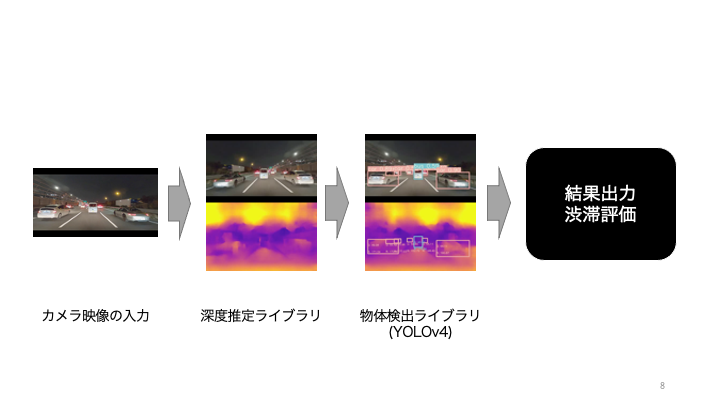
\includegraphics[width=15cm]{figs/system_net.png}
    \caption{ネットワークアーキテクチャ}
    \label{fig:system_arch}
  \end{center}
\end{figure}



\subsection{距離推定と深度推定ライブラリ}
ドライブレコーダー映像から車間距離を推定する方法は深度推定ライブラリを利用する方法がある.
本研究では深度推定ライブラリの中からFCRN-DepthPrediction\cite{laina2016deeper}とstruct2depth\cite{casser2019struct2depth}の2つをピックアップした.
どちらのライブラリもは入力された映像から奥行きを推定し,カメラとの距離を色の明暗によって塗り分けがされる.
本研究ではそのシステムを利用し,自動車が検出されたBBOXの場所と同期させることでその明るさから先行車との車間距離を推定する.
また,ピックアップした2つのライブラリのどちらかを使用するかについては実装と予備実験の項にて実験を行い,決定する.

% 自動車の検出について---
\subsection{自動車検出}
自動車の検出には物体検出ライブラリを使用する.
物体検出を行うライブラリは様々あり,Fast R-CNNs,Mask R-CNNs,SSDといった手法が挙げられる.
それぞれCNNと呼ばれる畳み込みネットワークを利用し物体検出を行なっている点は同じだが,そのCNNの層や物体検出を行う際の手法がわずかながらに異なっている.
本研究では物体検出手法としてYOLO(You Only Look Once)と呼ばれる物体検出手法を用いる.
このシステムは物体を検出するとその物体をBounding Box(BBOX)と呼ばれる四角形で囲むことでその物体の映像における位置を示すものである.
YOLOは上記の3つの手法と比較して畳み込みネットワークやニューラルネットワークがシンプルな構造になっているにもかかわらず,高い検出率を誇っている.
また,構造が比較的シンプルなため演算処理にかかるスピードが速く,リアルタイムでの処理にも適している.
本研究では,YOLOがMicrosoft COCO datasetを学習したものを利用する.


\section{渋滞の判断}
背景の項でも述べた通り,日本において渋滞の定義は自動車の運行スピードに依存しているが,本研究においては正確なスピードを取得するのは困難なため,先行車との車間距離を推定することで,その推定された距離を元に渋滞しているかどうかを判断する.

%\begin{figure}[htbp]
%  \begin{center}
%    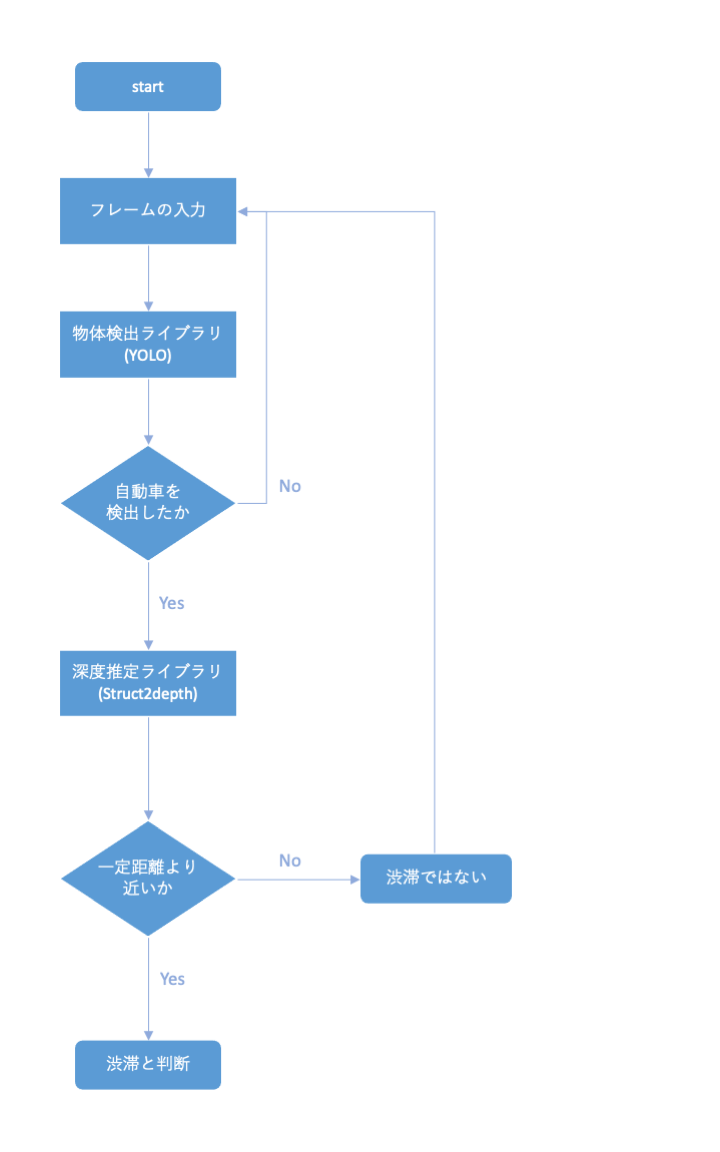
\includegraphics[width=9cm]{figs/gp2_flowchart.png}
%    \caption{フローチャート}
%    \label{fig:system_flow}
%    このフローチャートでは本研究が提案する渋滞推定システムのプロセスを簡略的に示す.
%渋滞検出システムでは入力された動画の各フレームを処理する.
%    まず,入力された映像の各フレームは物体検出ライブラリYOLOによって物体検出が行われる.
%ここで自動車が検出されなければ,次のフレームが処理される.
%    自動車が検出されると,次は深度推定ライブラリ(struct2depth)によって深度推定が行われる.
%    そして推定された距離が一定値より少ないと,システムは渋滞と判断し,それ以外は渋滞ではないと判断される.
%  \end{center}
%\end{figure}